% Ensure that you compile using XeLaTeX !!! PDFTex has problems with some of the packages used
\documentclass[12pt]{article}
\setlength\parindent{0pt}

\usepackage{parskip}
\usepackage[margin=0.5in]{geometry}
\usepackage{fullpage}
\usepackage{moresize}
\usepackage{graphicx}
\usepackage{caption}
\usepackage{subcaption}
\usepackage{float}
\usepackage{xcolor}
\usepackage{soul}
\usepackage{fontspec}
\setmainfont{Doulos SIL}

\begin{document}

\begin{center}
\textbf{{\color{violet}{\HUGE 20201110 Tuesday\\}}}

\textbf{{\color{violet}{\HUGE ALL EXAMS (with notes)\\}}}

\end{center}
\newpage

\begin{center}
\textbf{{\color{blue}{\HUGE START OF EXAM\\}}}

\textbf{{\color{blue}{\HUGE Student ID: 29164\\}}}

\textbf{{\color{blue}{\HUGE 9:00\\}}}

\end{center}
\newpage

{\large Question 1}\\

Topic: Articulatory Phonetics\\
Source: Homework 1, Question 3(a)\\

Could this image be the result of producing the sound represented by the given IPA symbol? Why or why not?\\

{[d]}

\begin{figure}[H]
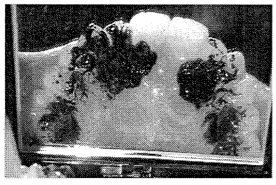
\includegraphics{../images/staticpalatography_fricative.png}
\end{figure}

~\\
INSTRUCTOR NOTES: no; space


\vfill
Excellent (3) ~~~ Good (2.2) ~~~ Fair (1.7) ~~~ Poor (0)
\newpage

{\large Question 2}\\

Topic: Phonological Features\\
Source: Quiz 3, Question 3\\

Explain why this featural specification either does or does not match the given sound.\\

{[-consonantal]}, {[+sonorant]}

{[h]}


~\\
INSTRUCTOR NOTES: does not match: [h] is [-cons] but also [-son], because its constriction is in the larynx, not the vocal tract


\vfill
Excellent (3) ~~~ Good (2.2) ~~~ Fair (1.7) ~~~ Poor (0)
\newpage

\begin{center}
\textbf{{\color{red}{\HUGE END OF EXAM}}}\\

\end{center}
\newpage

\begin{center}
\textbf{{\color{blue}{\HUGE START OF EXAM\\}}}

\textbf{{\color{blue}{\HUGE Student ID: 17357\\}}}

\textbf{{\color{blue}{\HUGE 9:10\\}}}

\end{center}
\newpage

{\large Question 1}\\

Topic: Phonological Features\\
Source: Quiz 3, Question 12\\

Explain how you figure out which feature is involved in the process of umlaut shown below.\\

\begin{figure}[H]
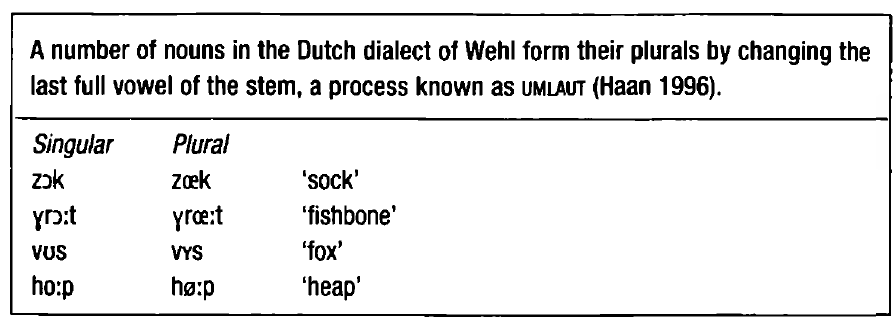
\includegraphics{../images/dutch.png}
\end{figure}

~\\
INSTRUCTOR NOTES: we look to see which vowels are affected, and compare them to see which feature is DIFFERENT (not e.g. what features they share); so since the vowels in the singular and plural are identical except that the singular forms are back and the plural are front, it's the feature [back] that is relevant / changing / involved (not e.g. the feature [round] just because all of the vowels are round)


\vfill
Excellent (3) ~~~ Good (2.2) ~~~ Fair (1.7) ~~~ Poor (0)
\newpage

{\large Question 2}\\

Topic: Other (pre-midterm)\\
Source: Homework 2, Question 2\\

What would this Klingon phrase below be in English? How do you know?\\

{[vɑdʒqʰoqʰvɑm]}

\begin{figure}[H]
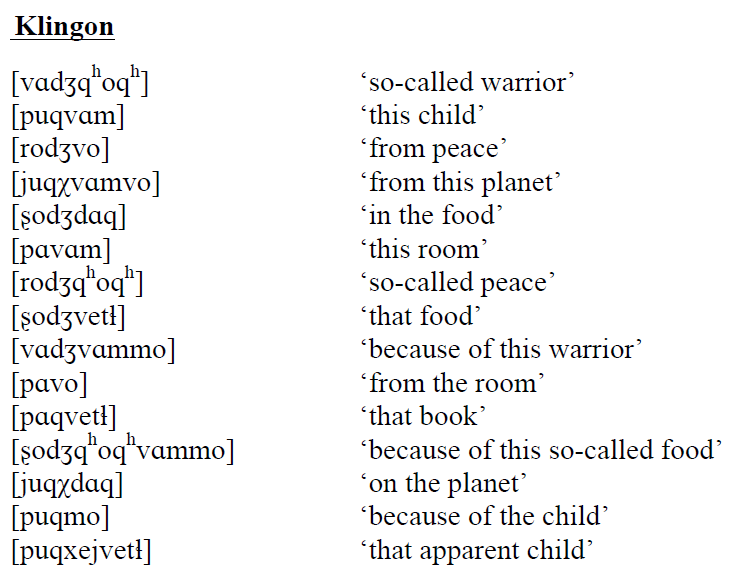
\includegraphics{../images/klingon.png}
\end{figure}

~\\
INSTRUCTOR NOTES: ‘this so-called warrior’


\vfill
Excellent (3) ~~~ Good (2.2) ~~~ Fair (1.7) ~~~ Poor (0)
\newpage

\begin{center}
\textbf{{\color{red}{\HUGE END OF EXAM}}}\\

\end{center}
\newpage

\begin{center}
\textbf{{\color{blue}{\HUGE START OF EXAM\\}}}

\textbf{{\color{blue}{\HUGE Student ID: 45517\\}}}

\textbf{{\color{blue}{\HUGE 9:20\\}}}

\end{center}
\newpage

{\large Question 1}\\

Topic: Skewed Distributions\\
Source: Week 5 Handout, Question 6\\

What would be a good description of the pattern in Malto? What characteristics make that a good description?\\

\begin{figure}[H]
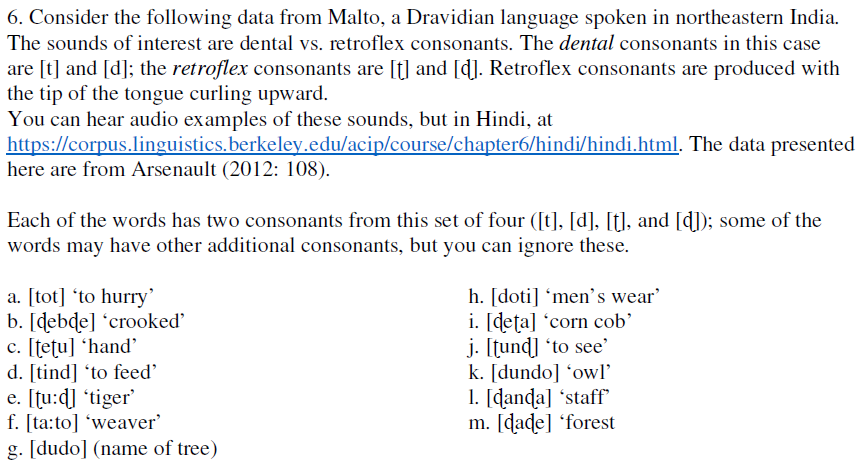
\includegraphics{../images/malto.png}
\end{figure}

~\\
INSTRUCTOR NOTES: It is not possible to have stops of different places of articulation co-occurring in a single word. Instead, if there are two stops, both must be dental, or both must be retroflex. For example, it’s possible to have a word with two dental stops, as in [tot] ‘to hurry’ (even if they disagree in voicing, as in [tind] ‘to feed’), or a word with two retroflex stops, as in [ɖebɖe] ‘crooked’ (again, regardless of voicing, as in [ɖeʈa] ‘corn cob’). But there are no words that have one dental and one retroflex stop, in either order, regardless of voicing. (accurate, generalizations, concrete examples)


\vfill
Excellent (3) ~~~ Good (2.2) ~~~ Fair (1.7) ~~~ Poor (0)
\newpage

{\large Question 2}\\

Topic: Transcription\\
Source: Week 2 Handout, Part II\\

Is this a reasonable transcription of this word? Explain why.\\

<climb>: {[klɑɪm]}


~\\
INSTRUCTOR NOTES: yes


\vfill
Excellent (3) ~~~ Good (2.2) ~~~ Fair (1.7) ~~~ Poor (0)
\newpage

\begin{center}
\textbf{{\color{red}{\HUGE END OF EXAM}}}\\

\end{center}
\newpage

\begin{center}
\textbf{{\color{blue}{\HUGE START OF EXAM\\}}}

\textbf{{\color{blue}{\HUGE Student ID: 37843\\}}}

\textbf{{\color{blue}{\HUGE 9:30\\}}}

\end{center}
\newpage

{\large Question 1}\\

Topic: Other (pre-midterm)\\
Source: Week 4 Handout, Part II, Question 2(iv)\\

Explain how you would figure out the Swahili word for this English gloss. (To be clear: you do NOT need to give me the Swahili form itself -- just explain the process of figuring it out.)\\

‘I like you (sg.).’

\begin{figure}[H]
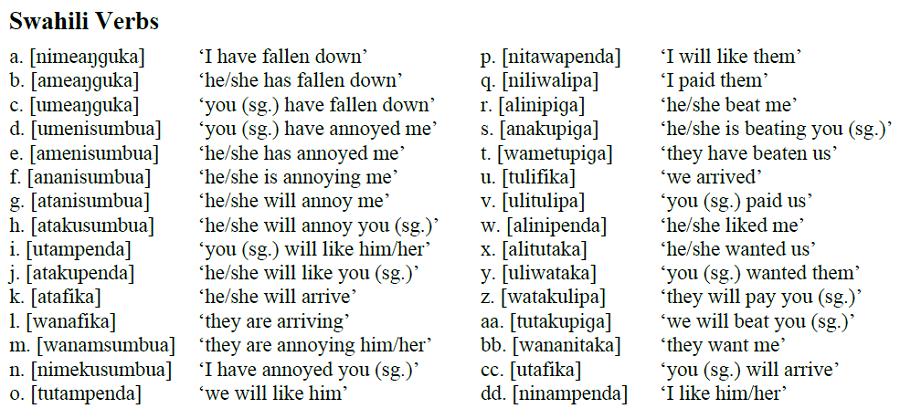
\includegraphics{../images/swahiliverbs.png}
\end{figure}

~\\
INSTRUCTOR NOTES: ([ninakupenda])


\vfill
Excellent (3) ~~~ Good (2.2) ~~~ Fair (1.7) ~~~ Poor (0)
\newpage

{\large Question 2}\\

Topic: Acoustics\\
Source: Week 9 Handout, Question 3\\

Explain what you see in the spectrogram that tells you about the properties of the sounds in the pictured word.\\

\begin{figure}[H]
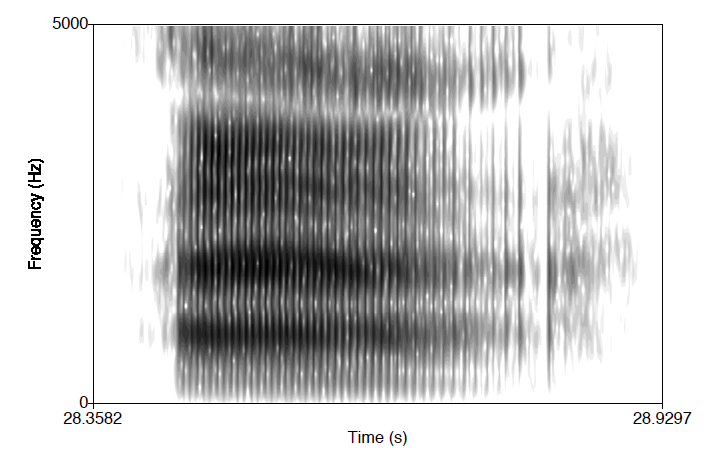
\includegraphics{../images/spectrogram_aaah.png}
\end{figure}

~\\
INSTRUCTOR NOTES: aaah: just a vowel; formants are very steady; F1 and F2 are pretty close to each other; F1 somewhat high and F2 somewhat low


\vfill
Excellent (3) ~~~ Good (2.2) ~~~ Fair (1.7) ~~~ Poor (0)
\newpage

\begin{center}
\textbf{{\color{red}{\HUGE END OF EXAM}}}\\

\end{center}
\newpage

\begin{center}
\textbf{{\color{blue}{\HUGE START OF EXAM\\}}}

\textbf{{\color{blue}{\HUGE Student ID: 17359\\}}}

\textbf{{\color{blue}{\HUGE 9:40\\}}}

\end{center}
\newpage

{\large Question 1}\\

Topic: Transcription\\
Source: Week 2 Handout, Part II\\

Is this a reasonable transcription of this word? Explain why.\\

<loud>: {[lɑud]}


~\\
INSTRUCTOR NOTES: okay, but [ɑʊ]


\vfill
Excellent (3) ~~~ Good (2.2) ~~~ Fair (1.7) ~~~ Poor (0)
\newpage

{\large Question 2}\\

Topic: Skewed Distributions\\
Source: Week 5 Handout, Question 6\\

What would be a good description of the pattern in Malto? What characteristics make that a good description?\\

\begin{figure}[H]
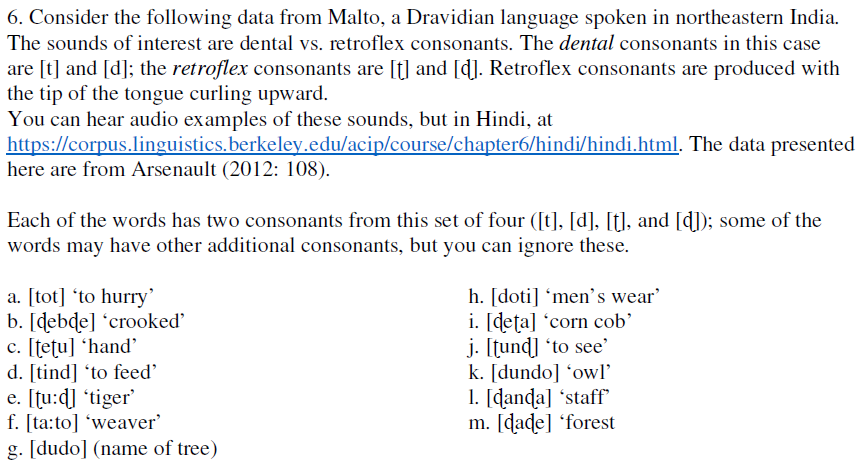
\includegraphics{../images/malto.png}
\end{figure}

~\\
INSTRUCTOR NOTES: It is not possible to have stops of different places of articulation co-occurring in a single word. Instead, if there are two stops, both must be dental, or both must be retroflex. For example, it’s possible to have a word with two dental stops, as in [tot] ‘to hurry’ (even if they disagree in voicing, as in [tind] ‘to feed’), or a word with two retroflex stops, as in [ɖebɖe] ‘crooked’ (again, regardless of voicing, as in [ɖeʈa] ‘corn cob’). But there are no words that have one dental and one retroflex stop, in either order, regardless of voicing. (accurate, generalizations, concrete examples)


\vfill
Excellent (3) ~~~ Good (2.2) ~~~ Fair (1.7) ~~~ Poor (0)
\newpage

\begin{center}
\textbf{{\color{red}{\HUGE END OF EXAM}}}\\

\end{center}
\newpage

\begin{center}
\textbf{{\color{blue}{\HUGE START OF EXAM\\}}}

\textbf{{\color{blue}{\HUGE Student ID: 38755\\}}}

\textbf{{\color{blue}{\HUGE 9:50\\}}}

\end{center}
\newpage

{\large Question 1}\\

Topic: Articulatory Phonetics\\
Source: Homework 1, Question 3(a)\\

Could this image be the result of producing the sound represented by the given IPA symbol? Why or why not?\\

{[t͡ʃ]}

\begin{figure}[H]
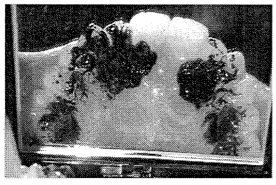
\includegraphics{../images/staticpalatography_fricative.png}
\end{figure}

~\\
INSTRUCTOR NOTES: no


\vfill
Excellent (3) ~~~ Good (2.2) ~~~ Fair (1.7) ~~~ Poor (0)
\newpage

{\large Question 2}\\

Topic: Other (pre-midterm)\\
Source: Homework 2, Question 2\\

What would this Klingon phrase below be in English? How do you know?\\

{[pɑdɑq]}

\begin{figure}[H]
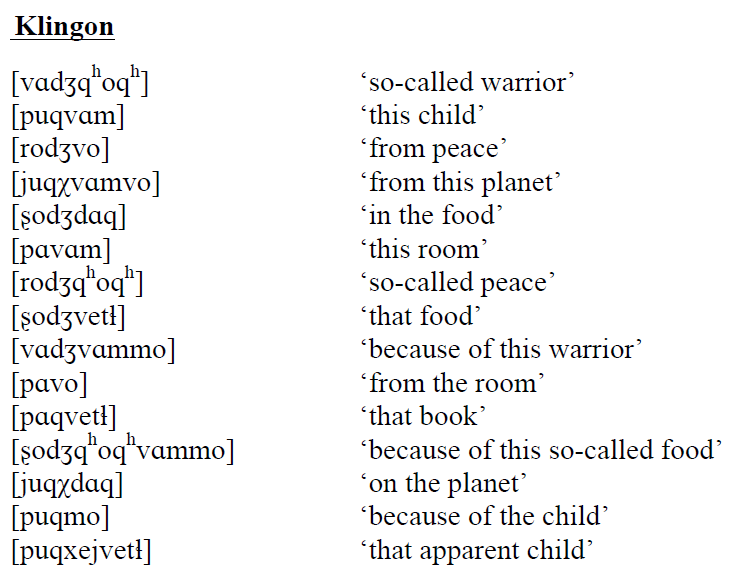
\includegraphics{../images/klingon.png}
\end{figure}

~\\
INSTRUCTOR NOTES: ‘in/on (the) room’


\vfill
Excellent (3) ~~~ Good (2.2) ~~~ Fair (1.7) ~~~ Poor (0)
\newpage

\begin{center}
\textbf{{\color{red}{\HUGE END OF EXAM}}}\\

\end{center}
\newpage

\end{document}

